%----------------------------------------------------------------------------
\chapter{\github}
%----------------------------------------------------------------------------
\section{Git}
A verziókezelő rendszer (későbbiekben Version Control System vagy VCS) nyomon követi a változtatások történetét, ahogy az emberek és a csapatok együtt dolgoznak a projekteken.
Ahogy a fejlesztők változtatásokat végeznek a projekten, a projekt bármely korábbi verziója bármikor visszaállítható.

A fejlesztők áttekinthetik a projekttörténetet, hogy megtudják:
\begin{itemize}
  \item Milyen változtatásokat végeztek.
  \item Ki végezte a változtatásokat.
  \item Mikor történtek a változtatások.
  \item Miért volt szükség a változtatásokra.
\end{itemize}

A VCS-ek minden egyes közreműködőnek egységes és konzisztens képet adnak a projektről, felszínre hozva a már folyamatban lévő munkát.
A változtatások átlátható előzményeinek, a változtatásokat végző személyeknek és a projekt fejlődéséhez való hozzájárulásuknak a megtekintése segít a csapattagoknak abban, hogy a független munka során is összhangban maradjanak.

Egy elosztott verziókezelő rendszerben (későbbiekben Distributed Version Control System vagy DVCS) minden fejlesztő rendelkezik a projekt és a projekttörténet teljes másolatával.
Az egykor népszerű központosított verziókezelő rendszerekkel ellentétben a DVCS-eknek nincs szükségük állandó kapcsolatra egy központi adattárral.

\newpage

A Git a legnépszerűbb elosztott verziókezelő rendszer. A Git-et gyakran használják nyílt forráskódú és kereskedelmi szoftverfejlesztésre egyaránt, és jelentős előnyökkel jár az egyének, a csapatok és a vállalkozások számára:
\begin{itemize}
  \item A Git segítségével a fejlesztők egy helyen láthatják a változtatások, döntések és a projekt előrehaladásának teljes idővonalát. Attól a pillanattól kezdve, hogy hozzáférnek egy projekt előzményeihez, a fejlesztő minden szükséges kontextussal rendelkezik ahhoz, hogy megértse azt, és elkezdjen hozzájárulni.
  \item A fejlesztők minden időzónában dolgoznak. Egy olyan DVCS-vel, mint a Git, az együttműködés bármikor megtörténhet, miközben a forráskód integritása megmarad. Az ágak használatával a fejlesztők biztonságosan javasolhatnak változtatásokat a termelési kódhoz.
  \item A Git-et használó vállalkozások lebonthatják a csapatok közötti kommunikációs akadályokat, és a csapatok a legjobb munkájukra koncentrálhatnak. Ráadásul a Git lehetővé teszi, hogy az egész vállalat szakértői együttműködjenek a nagyobb projektekben.
\end{itemize}

A repository vagy Git-projekt a projekthez tartozó fájlok és mappák teljes gyűjteményét foglalja magában, az egyes fájlok revíziós előzményeivel együtt.
A fájlok előzményei időbeli pillanatképek formájában jelennek meg, amelyeket commitoknak nevezünk.
A commitok több fejlesztési sorba, úgynevezett ágakba szervezhetők. Mivel a Git egy DVCS, a tárolók önálló egységek, és bárki, aki rendelkezik a tároló másolatával, hozzáférhet a teljes kódbázishoz és annak történetéhez.
A parancssor vagy más egyszerű kezelőfelületek használatával a Git-tár lehetővé teszi a következőket is: interakció az előzményekkel, a tár klónozása, ágak létrehozása, átadás, beolvasztás, összevonás, a kódverziók közötti változások összehasonlítása stb.

Az olyan platformokon keresztül, mint a GitHub, a Git több lehetőséget biztosít a projektek átláthatóságára és együttműködésére is.
A nyilvános adattárak segítik a csapatok együttműködését a lehető legjobb végtermék létrehozásában \cite{git}.

\section{GitHub}
A GitHub egy olyan fejlesztési platform, amely lehetővé teszi a kódok tárolását és felülvizsgálatát, a projektek kezelését és a szoftverek készítését 50 millió fejlesztővel együttműködve.
Miért épít mindenki a GitHubra? Mert biztosítja azokat a fontos DevOps funkciókat, amelyekre a vállalatoknak és a különböző méretű szervezeteknek szükségük van a nyilvános és magánprojektjeikhez.
Legyen szó funkciók tervezéséről, hibák javításáról vagy a változtatásokon való együttműködésről, a GitHub az a hely, ahol a világ szoftverfejlesztői összegyűlnek, hogy dolgokat hozzanak létre és aztán jobbá teszik őket.
A GitHub egy felhőplatform, amely a Git-et használja alapvető technológiaként.
Leegyszerűsíti a projekteken való együttműködés folyamatát, és olyan weboldalt, parancssori eszközöket és általános folyamatot biztosít, amely lehetővé teszi a fejlesztők és a felhasználók közös munkáját.

\subsection{GitHub Actions ismertető}
A GitHub Actions egy folyamatos integrációs és folyamatos szállítási (későbbiekben CI/CD) platform, amely lehetővé teszi, hogy automatizálja a build, a tesztelés és a telepítés folyamatot.
Létrehozhat olyan munkafolyamatokat (későbbiekben workflow), amelyek minden egyes pull-kérelem után build-el és tesztel a tárolóban (későbbiekben repository).

A GitHub Actions túlmutat a DevOps-on, és lehetővé teszi, hogy workflow-kat futtasson, amikor más események is történnek a tárolóban.
Például futtathat olyan workflow-t, amely automatikusan hozzáadja a megfelelő címkéket, amikor valaki új problémát (későbbiekben issue) hoz létre az respository-ban.

A GitHub Linux, Windows és macOS virtuális gépeket biztosít a workflow-ok futtatásához, de saját adatközpontban vagy felhő-infrastruktúrában is hosztolhatsz saját, saját üzemeltetésű futásokat (későbbiekben runner) \cite{github}.

\subsection{A GitHub Actions elemei}
Konfigurálhat egy GitHub Actions workflow-t, amely akkor indul el, amikor egy esemény történik a repository-ban, például egy pull request megnyitásakor vagy egy issue létrehozásakor.
A workflow egy vagy több feladatot tartalmaz, amelyek futhatnak egymás utáni sorrendben vagy párhuzamosan (lásd \ref{overview-actions-simple} ábrán).
Minden egyes feladat a saját virtuális gépi runner-jén vagy egy konténeren belül fut, és egy vagy több lépésből áll, amelyek vagy egy általad definiált szkriptet futtatnak, vagy egy műveletet futtatnak, ami egy újrafelhasználható bővítmény, amely egyszerűsítheti a workflow-t \cite{github}.

\begin{figure}[ht]
    \centering
         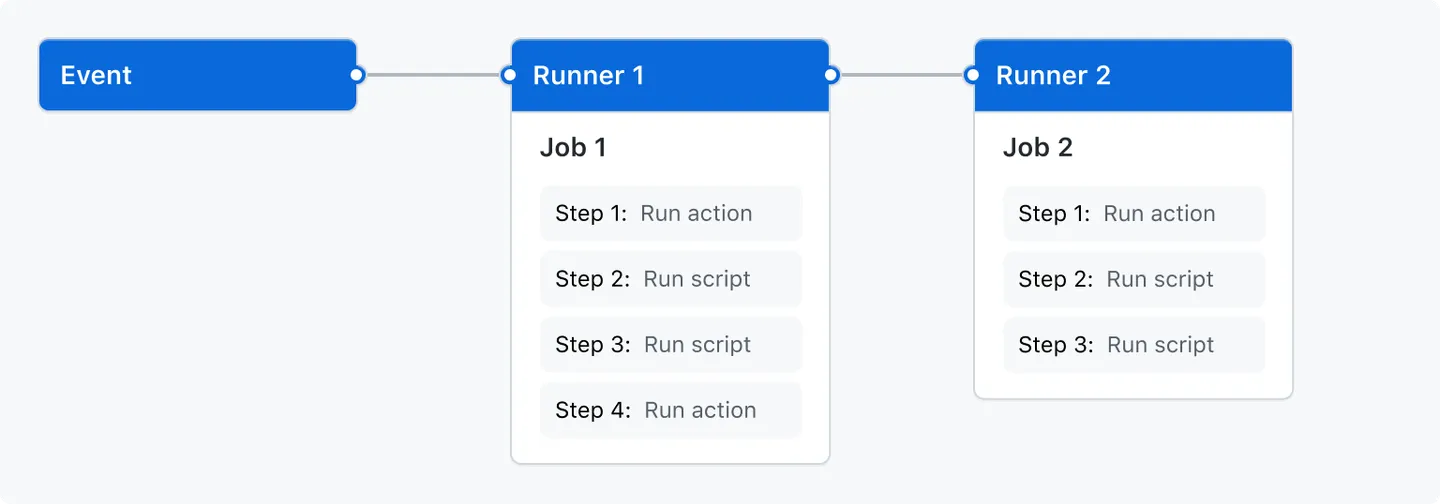
\includegraphics[width=1.0\textwidth]{figures/github/overview-actions-simple.png}
          \caption{Egy esemény diagramja, amely az 1. runner-t az 1. feladat futtatására indítja, ami a 2. runner-t a 2. feladat futtatására indítja. Mindegyik feladat több lépésre van bontva \cite{github}.}
           \label{overview-actions-simple}
\end{figure}

\subsubsection*{Workflows}
A workflow egy konfigurálható automatizált folyamat, amely egy vagy több feladatot futtat. A workflow-kat az repository-ba bevitt YAML fájl határozza meg, és akkor futnak, amikor az repository-ban lévő esemény kiváltja őket, vagy manuálisan, illetve meghatározott ütemezés szerint is elindíthatók.

A workflow-k a .github/workflows könyvtárban vannak definiálva egy repository-ban, és egy repository-hoz több workflow is tartozhat, amelyek mindegyike más-más feladatokat végezhet.
Például lehet egy workflow a pull-kérelmek létrehozására és tesztelésére, egy másik workflow az alkalmazás telepítésére minden egyes kiadás létrehozásakor, és még egy másik workflow, amely minden egyes alkalommal hozzáad egy címkét, amikor valaki új issue-t nyit. Hivatkozhat egy workflow-ra egy másik workflow-on belül \cite{github}.

\subsubsection*{Events}
Az esemény (event) egy konkrét tevékenység egy repository-ban, amely egy workflow végrehajtását indítja el.
Az aktivitás például a GitHubról származhat, amikor valaki létrehoz egy pull requestet, megnyit egy issue-et, vagy egy commit-ot küld a repositoryba. A workflow-t időzítéssel, REST API-ba való beküldéssel vagy manuálisan is elindíthatja \cite{github}.

\subsubsection*{Jobs}
A feladat (job) egy workflow lépéseinek olyan csoportja, amelyet ugyanazon a runner-en hajtanak végre.
Minden lépés vagy egy végrehajtandó shell szkript, vagy egy végrehajtandó művelet.
A lépések sorrendben kerülnek végrehajtásra, és egymástól függnek. Mivel minden lépés ugyanazon a futón kerül végrehajtásra, az adatokat megoszthatja egyik lépésről a másikra. Például lehet egy lépés, amely elkészíti az alkalmazást, majd egy lépés, amely teszteli a felépített alkalmazást.

Beállíthatja egy feladat függőségeit más feladatokkal; alapértelmezés szerint a feladatoknak nincsenek függőségeik, és párhuzamosan futnak egymással.
Ha egy feladat függőséget vesz fel egy másik feladattól, akkor megvárja a függő feladat befejezését, mielőtt lefuthatna. Lehet például több, különböző architektúrákhoz tartozó építési feladat, amelyek nem függnek egymástól, és egy csomagolási feladat, amely függ ezektől a feladatoktól.
A build feladatok párhuzamosan futnak, és ha mindegyik sikeresen befejeződött, akkor a csomagolási feladat is lefut \cite{github}.

\subsubsection*{Actions}
A művelet (action) a GitHub Actions platform egyéni alkalmazása, amely egy összetett, de gyakran ismétlődő feladatot hajt végre.
Egy művelet használatával csökkentheti a workflow fájlokban írt ismétlődő kód mennyiségét.
Egy művelet lehívhatja a git-tárat a GitHubról, beállíthatja a megfelelő eszköztárat az build környezetéhez, vagy beállíthatja a hitelesítést a felhőszolgáltatónál.

Írhat saját műveleteket, vagy találhat workflow-okhoz felhasználható műveleteket a GitHub Marketplace-en \cite{github}.

\subsubsection*{Runners}
A futtató (későbbiekben runner) egy olyan kiszolgáló, amely a workflow-okat futtatja, amikor azoknak el kell elindulniuk.
Minden runner egyszerre egyetlen feladatot futtathat.
A GitHub Ubuntu Linux, Microsoft Windows és macOS runnereket biztosít a workflow-ok futtatásához; minden workflow futtatása egy friss, újonnan rendelkezésre bocsátott virtuális gépen történik.
A GitHub nagyobb futókat is kínál, amelyek nagyobb konfigurációkban állnak rendelkezésre \cite{github}.

\subsubsection*{Egy példa workflow}
A GitHub Actions YAML szintaxist használ a workflow-ok meghatározásához.
Minden workflow különálló YAML-fájlként tárolódik a kódtárában, a .github/workflows nevű könyvtárban.

Létrehozhat egy példát a repository-jában ahogyan a \ref{sample-actions-config} ábrán is látható, amely automatikusan elindít egy sor parancsot, amikor kódot küldünk be.
Ebben a workflow-ban a GitHub Actions ellenőrzi a beküldött kódot, telepíti a bats tesztelési keretrendszert, és lefuttat egy alapvető parancsot a bats verziójának kiadására: bats -v \cite{github}.

\begin{figure}
  \centering
    \begin{minipage}{\linewidth}
      \begin{lstlisting}
          name: learn-github-actions
          run-name: ${{ github.actor }} is learning GitHub Actions
          on: [push]
          jobs:
            check-bats-version:
              runs-on: ubuntu-latest
              steps:
                - uses: actions/checkout@v3
                - uses: actions/setup-node@v3
                  with:
                    node-version: '14'
                - run: npm install -g bats
                - run: bats -v
      \end{lstlisting}
      \end{minipage}
  \caption{Példa kód a GitHub Actions használatára \cite{github}.}
  \label{sample-actions-config}
\end{figure}

A \ref{overview-actions-event} ábrán látható az imént létrehozott példa workflow fájl, valamint a GitHub Actions összetevőinek hierarchikus elrendezése.
Minden lépés egyetlen műveletet vagy szkriptet hajt végre.
Az 1. és 2. lépés műveleteket, míg a 3. és 4. lépés szkripteket futtat.

\begin{figure}[ht]
    \centering
         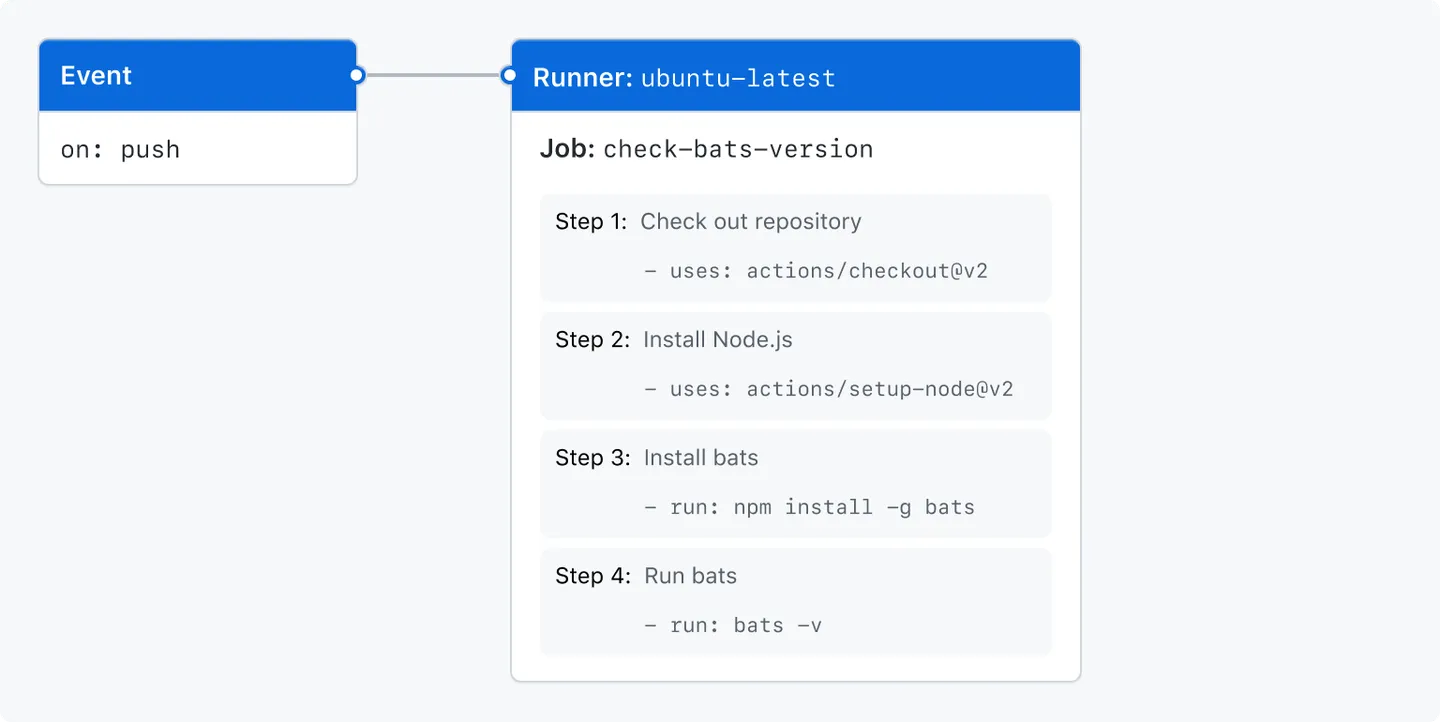
\includegraphics[width=0.95\textwidth]{figures/github/overview-actions-event.png}
          \caption{Egy workflow triggerét, runner-ét és feladatát bemutató ábra. A feladat 4 lépésre van bontva \cite{github}.}
           \label{overview-actions-event}
\end{figure}